\documentclass[a4paper,12pt]{article}

% Preamble einbinden
% --- Sprache und Kodierung ---
\usepackage[utf8]{inputenc}
\usepackage[T1]{fontenc}
\usepackage[ngerman]{babel}

% --- Layout ---
\usepackage[a4paper,margin=2.5cm]{geometry}
\usepackage{setspace} % Zeilenabstand
\onehalfspacing
\usepackage{placeins} % Floatbarrier (Kapitel)

% --- Schriftarten ---
\usepackage{lmodern}

% --- Mathe und Symbole ---
\usepackage{amsmath, amssymb, amsthm}
\usepackage{calc}

% --- Grafiken ---
\usepackage{graphicx}
\usepackage{tcolorbox}
\tcbset{
    myboxstyle/.style={
        colframe=blue!60!black,      % border color
        colback=blue!5,              % light background color
        boxrule=1pt,                 % border thickness
        arc=2mm,                     % rounded corners (optional)
        left=3pt,right=3pt,top=3pt,bottom=3pt, % padding
        width=\textwidth,
        fontupper=\footnotesize
    }
}
\usepackage{float} % bessere Kontrolle von Abbildungen
\graphicspath{{figures/}}

% --- Tabellen ---
\usepackage{booktabs}
\usepackage{threeparttable}
\usepackage{tabularx}
\usepackage{makecell}
\usepackage{booktabs}
\usepackage{siunitx}
\usepackage{multicol}
\usepackage{multirow}
\usepackage[table]{xcolor}
\sisetup{
    detect-all,
    table-format=3.2,
    separate-uncertainty = true,
    output-decimal-marker = {.}
}

% --- Referenzen und Links ---
\usepackage[hidelinks]{hyperref}
\usepackage{cleveref}
% Deutsche Bezeichnungen für \cref/\Cref
\crefname{figure}{Abbildung}{Abbildungen}
\Crefname{figure}{Abbildung}{Abbildungen}
\crefname{table}{Tabelle}{Tabellen}
\Crefname{table}{Tabelle}{Tabellen}
\crefname{equation}{Gleichung}{Gleichungen}
\Crefname{equation}{Gleichung}{Gleichungen}
\usepackage[labelfont=bf,font={footnotesize, it},labelsep=colon]{caption}
\usepackage[backend=biber,style=apa]{biblatex}
\addbibresource{bibliography.bib}
% Required for APA style
\DeclareLanguageMapping{english}{english-apa}


% --- Sonstiges ---
\usepackage{xcolor}
\usepackage{csquotes} % für saubere Zitate
\setlength{\marginparwidth}{2cm}
\usepackage[textsize=tiny]{todonotes}
\usepackage{ifthen}
\usepackage{xkeyval}
\usepackage{tikz}
\usepackage{lscape}
\usepackage{pdflscape}

\setcounter{tocdepth}{2}

\begin{document}

% Titelseite
\parindent 0mm
\begin{titlepage}
    \begin{figure}[t]
        \centering
        
\includegraphics[width=16cm]{fhnw_habg_igeo_10mm.jpg}
    \end{figure}

    \vspace*{1.5cm}

    \begin{center}
        \textsf{
            \textbf{\LARGE Titel des Berichtes}\\[1cm]
            {\LARGE Untertitel Bericht}
        }
        \vspace{0.5cm}
    \end{center}

    \begin{figure}[h]
        \centering
        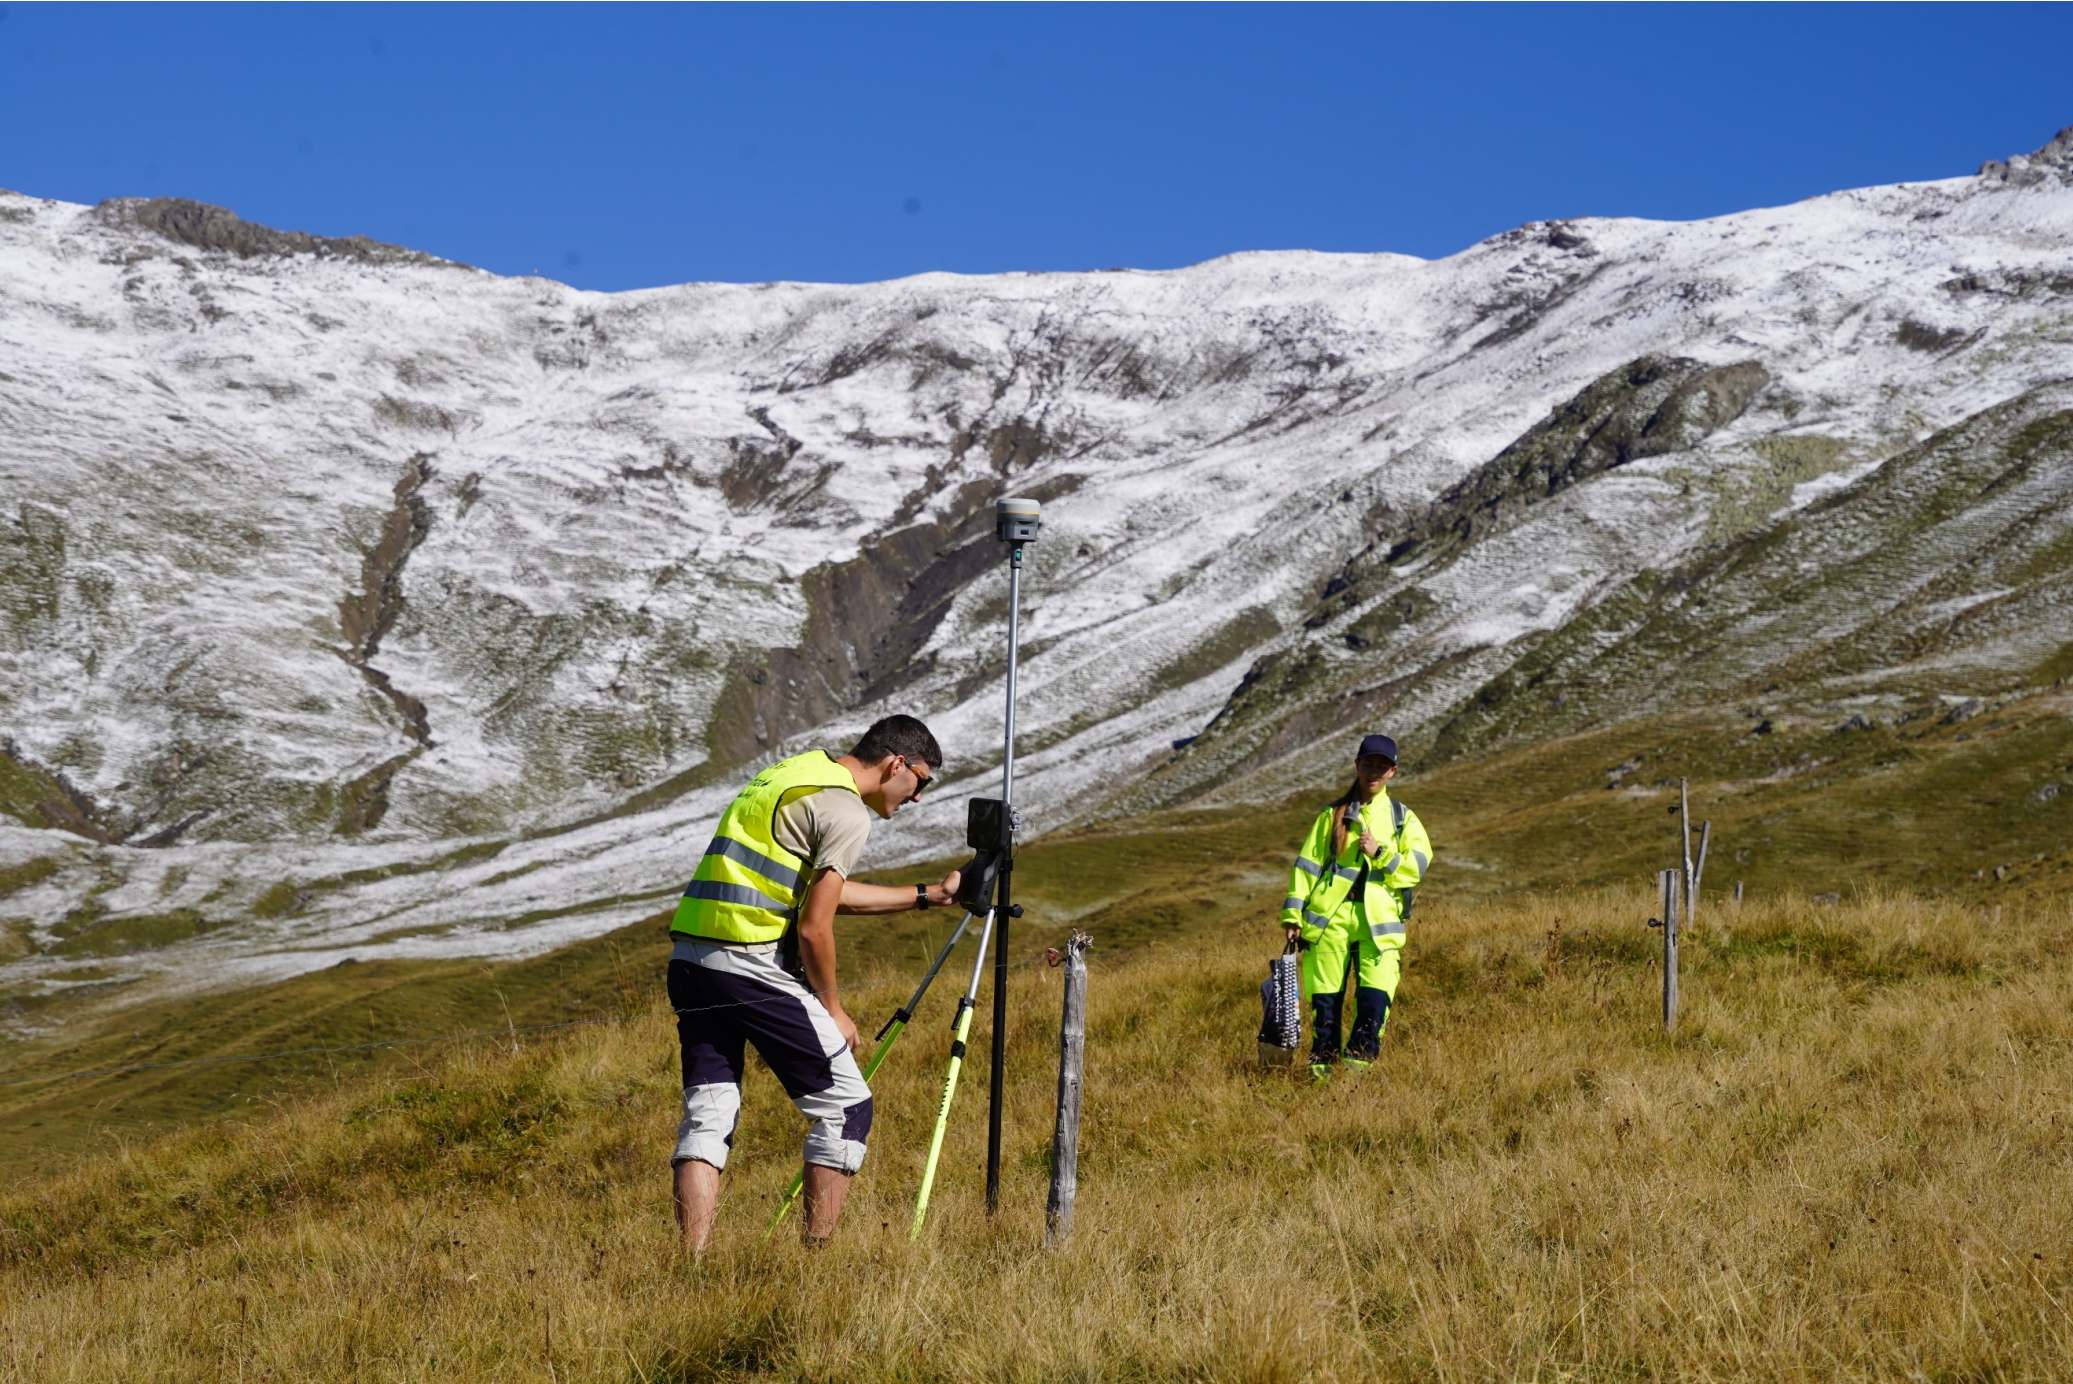
\includegraphics[width=14cm]{gnss_mountains.jpg}
    \end{figure}

    \vfill  % pushes the following text to the bottom

    \begin{flushleft}
        \textsf{
            \text{ }\\
            \textbf{Gruppe 1}\\[0.1cm]
            \textbf {Verantwortlicher Autor}\\
            Autorin zwei\\
            Autor Drei\\
            Autor vier\\[0.5cm]
            Eingereicht bei: Betreuende - Modul Modulname\\
            \textbf{\today}\\
        }
    \end{flushleft}
\end{titlepage}


\newpage
\thispagestyle{empty}
\null
\vfill
%\pagenumbering{Roman}
\footnotesize{\textbf{Abbildung Titelseite:} Bildtext Titelbild, allenfalls Quelle} \\[2cm]
Version X.X                                   \\[1cm]
Fachhochschule Nordwestschweiz (FHNW)         \\
Hochschule für Architektur, Bau und Geomatik  \\
Institut Geomatik                             \\
Hofackerstrasse 30                            \\
CH-4132 Muttenz                               \\
 
\verb"https://www.fhnw.ch"                   \\

\cleardoublepage
\tableofcontents
\newpage
\listoffigures
\listoftables
\newpage



% Kapitel laden
\clearpage
\section{Einleitung}

Lorem ipsum dolor sit amet, consectetur adipiscing elit. Pellentesque lobortis pretium urna et gravida. Nunc ornare, 
ex id dictum dapibus, felis purus pulvinar erat, sed semper est metus eu turpis. Phasellus feugiat nisi massa, vehicula 
tincidunt ipsum scelerisque id. Nam sem eros, venenatis vel sapien quis, rhoncus pellentesque nulla. Nullam eget dolor
 tortor. Aliquam quis massa ut metus auctor tempus et imperdiet lacus. Curabitur bibendum sagittis efficitur. In vitae 
 tristique ex, eget fringilla libero. Aliquam ullamcorper semper congue. Donec ac arcu ut quam posuere tempor ac nec metus.

\subsection{Zielsetzung}
Dies ist eine Aufzählung:
\begin{itemize}
    \item 1 Punkt.
    \item 2 Punkt.
    \item ...
\end{itemize}

\input{chapters/02_methodik.tex}
\section{Resultate}
\label{sec:resultate}

\subsection{Beispiel mit farbig hervorgehobener Tabelle}
\label{subsec:beispiel-farbtabelle}
Mit dem Paket \texttt{xcolor} (Option \texttt{table}) können einzelne Tabellenzeilen
hervorgehoben werden, siehe Tabelle~\ref{tab:beispiel-farbtabelle}.

\begin{table}[h!]
    \centering
    \caption{Beispieltabelle mit farbig hervorgehobenen Zeilen.}
    \label{tab:beispiel-farbtabelle}
    \begin{tabularx}{\textwidth}{l *{2}{>{\centering\arraybackslash}X}}
        \toprule
        \textbf{Punktnr.} & \textbf{Abweichung [cm]} & \textbf{Bemerkung} \\
        \midrule
        1001 & 1.2 & Platzhalter \\
        \rowcolor{lightgray}
        1002 & 3.4 & \textcolor{red}{\textbf{Auffälliger Wert}} \\
        1003 & 0.8 & Platzhalter \\
        \bottomrule
    \end{tabularx}
\end{table}

\subsection{Beispiel einer mehrspaltigen Liste}
\label{subsec:beispiel-multicol}
Mit dem Paket \texttt{multicol} können Aufzählungen auf mehrere Spalten verteilt werden,
zum Beispiel für Listen mit vielen kurzen Einträgen: \todo{Dies ist ein To-do Kommentar}

\begin{multicols}{2}
    \begin{itemize}
        \item Eintrag 1
        \item Eintrag 2
        \item Eintrag 3
        \item Eintrag 4
        \item Eintrag 5
        \item Eintrag 6
    \end{itemize}
\end{multicols}

\subsection{Beispiel eines einfachen Diagramms}
\label{subsec:beispiel-tikz}
Mit dem Paket \texttt{tikz} können einfache Diagramme direkt in \LaTeX{} erstellt werden,
siehe \Cref{fig:beispiel-tikz}.

\begin{figure}[h!]
    \centering
    \begin{tikzpicture}
        \node[draw, rectangle, minimum width=2.5cm, minimum height=1cm] (a) at (0,0) {Schritt 1};
        \node[draw, rectangle, minimum width=2.5cm, minimum height=1cm] (b) at (4,0) {Schritt 2};
        \draw[->] (a) -- (b);
    \end{tikzpicture}
    \caption{Beispiel für ein einfaches \texttt{tikz}-Diagramm.}
    \label{fig:beispiel-tikz}
\end{figure}

\FloatBarrier
\section{Diskussion}
\label{sec:diskussion}

Dies ist Platzhaltertext für die Diskussion der Resultate. Hier werden die in
Kapitel~\ref{sec:resultate} vorgestellten Ergebnisse eingeordnet und kritisch bewertet.

\subsection{Beispiel für Querverweise}
\label{subsec:querverweise}
Mit dem Paket \texttt{cleveref} können Querverweise automatisch mit dem passenden Typ
beschriftet werden, zum Beispiel ein Verweis auf \Cref{tab:beispieltabelle} oder auf
\Cref{fig:beispielbild}. Ebenso kann erneut auf eine Quelle verwiesen werden
\cite{muster_beispielquelle_2025}.

\subsection{Einschränkungen}
\label{subsec:einschraenkungen}
Dies ist Platzhaltertext für die Beschreibung von Einschränkungen oder offenen Fragen.

\section{Fazit}
\label{sec:fazit}

Dies ist Platzhaltertext für das Fazit. Hier werden die wichtigsten Erkenntnisse des
Berichts kurz zusammengefasst und ein Ausblick auf allfällige weitere Schritte gegeben.



% Literatur
\newpage
\section{Quellenverzeichnis}
\printbibliography

\section{Anhang}
\label{sec:anhang}

Dies ist Platzhaltertext für den Anhang, zum Beispiel eine Liste der beigelegten
Dokumente:
\begin{itemize}
    \item 01\_Beispieldokument
    \item 02\_Beispieldokument
\end{itemize}

\subsection{Beispiel einer verschachtelten Datenstruktur}
\label{subsec:datenstruktur}
Verschachtelte Aufzählungen eignen sich zum Beispiel zur Darstellung einer
Ordnerstruktur:
\begin{itemize}
    \item Projektordner
    \begin{itemize}
        \item 10\_Rohdaten
        \begin{itemize}
            \item Beispieldatei\_1
            \item Beispieldatei\_2
        \end{itemize}
        \item 20\_Auswertung
        \item 30\_Ausgabe
    \end{itemize}
\end{itemize}


\end{document}
